 \documentclass{openetcs_report}
% Use the option "nocc" if the document is not licensed under Creative Commons
%\documentclass[nocc]{template/openetcs_article}
\usepackage{todonotes}
\usepackage{appendix}
\usepackage{lipsum,url}
\usepackage{pdfpages}
%\usepackage{bibtopic} % Multibib
\usepackage{booktabs}
\usepackage{hyperref}

\usepackage[section,                 % add the glossary to the table of content 
            description,             % acronyms have a user-supplied description,
            style=superheaderborder, % table style
            nonumberlist             % no page number
]{glossaries}
\hypersetup{
linkbordercolor 	={1 1 1}}

%===========================
% Graphicpath
%===========================
\graphicspath{{./template/}{.}{./images/}}

%===========================
% Abbreviation file
%===========================
% \renewcommand*{\glossaryname}{List of Terms}
% \makeglossaries
% \loadglsentries{wp7_glossary} 
%===========================
%===========================
% Todo note margin
%===========================
\setlength{\marginparwidth}{7em}
\let\oldmarginpar\marginpar
\renewcommand\marginpar[1]{\-\oldmarginpar[\raggedleft\footnotesize #1]%
{\raggedright\footnotesize #1}}
%===========================

\begin{document}

\frontmatter
\project{openETCS}

%Please do not change anything above this line
%============================
% The document metadata is defined below

%assign a report number here
\reportnum{OETCS/WP7/07.3.2}

%define your workpackage here
\wp{Work-Package 7: ``Toolchain''}

%set a title here
\title{OpenETCS Roadmap}

%set a subtitle here
%\subtitle{}

%set the date of the report here
\date{February 2014}

%define a list of authors and their affiliation here

\author{Cecile Braunstein}

\affiliation{University Bremen}



% define the coverart
\coverart[width=350pt]{openETCS_EUPL}

%define the type of report
\reporttype{OpenETCS : Tool Chain Roadmap}


\begin{abstract}
%define an abstract here
This document presents the OpenETCS tool chain Roadmap.
\end{abstract}


%=============================
%Do not change the next three lines
\maketitle
\tableofcontents
%\listoffiguresandtables

\newpage
%=============================

% The actual document starts below this line
%=============================
%Start here
%=============================
% Document Managment
%=============================
\chapter{Document Information}

\begin{tabular}{|p{4.4cm}|p{8.7cm}|}
\hline
\multicolumn{2}{|c|}{Document information} \\
\hline
Work Package &  WP7  \\
Deliverable ID or doc. ref. & O7.3.2\\
\hline
Document title & Toolchain Roadmap \\
Document version & 00.02 \\
Document authors (org.)  & Cécile Braunstein (Uni.Bremen) \\
\hline
\end{tabular}

\begin{tabular}{|p{4.4cm}|p{8.7cm}|}
\hline
\multicolumn{2}{|c|}{Review information} \\
\hline
Last version reviewed &  \\
\hline
Main reviewers &  \\
\hline
\end{tabular}

\begin{tabular}{|p{2.2cm}|p{4cm}|p{4cm}|p{2cm}|}
\hline
\multicolumn{4}{|c|}{Approbation} \\
\hline
  &  Name & Role & Date   \\
\hline  
Written by    &  Cécile Braunstein & WP7-T7.3 Sub-Task  & 06.02.2014 \\
&  & Leader&\\
\hline
Approved by &  &   &  \\
\hline
\end{tabular}

\begin{tabular}{|p{2.2cm}|p{2cm}|p{3cm}|p{5cm}|}
\hline
\multicolumn{4}{|c|}{Document evolution} \\
\hline
Version &  Date & Author(s) & Justification  \\
\hline  
00.00 & 06.02.2014 & C. Braunstein  &  Document creation  \\
00.01 & 10.02.2014 & C. Braunstein  &  Changes as suggested by MJ.\\
00.02 & 19.02.2014 & C. Braunstein  &  Chages as suggested by MPD. \\



\hline  
\end{tabular}
\newpage
%==========================================


%------ List of terms and definition ----------------
%\printglossary
%==========================================
\mainmatter
%----------------------







\chapter{OpenETCS Objectives}
\label{chap-1}
\section{Goals}
\label{sec-1-1}
One of the goals of the openETCS project is to {\em "Provide a tool chain and process/methodologies for developing an on-board software that can fulfill the CENELEC requirements for SIL4 software"}

The openETCS tool chain is the implementation of the design process of the on board unit (OBU)
according to the CENELEC EN 50128 depicted figure \ref{fig:lifecycle}.
\begin{figure}[htbp]
  \centering
  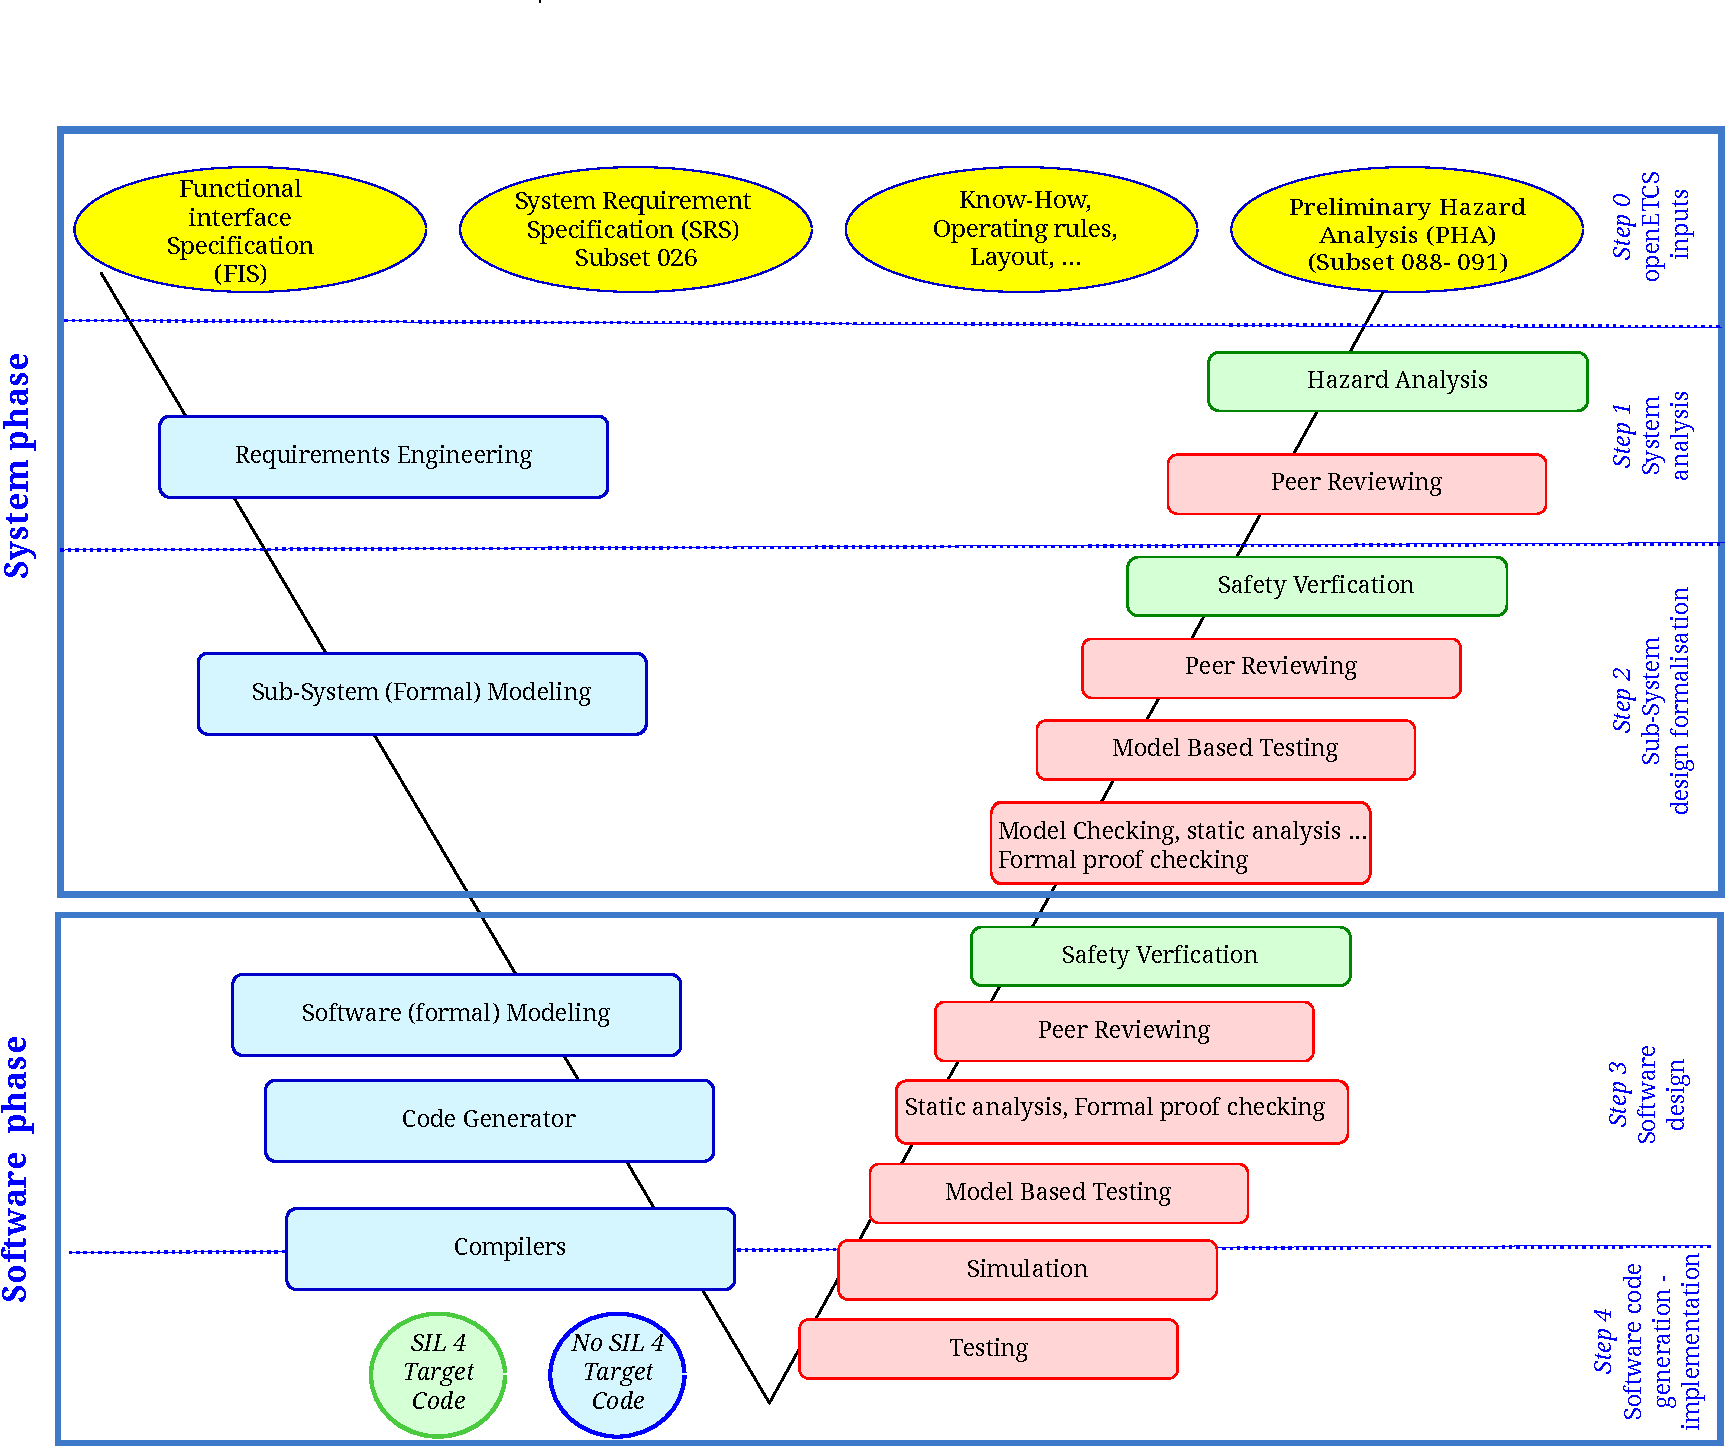
\includegraphics[width=\textwidth]{images/WholeProcess_Activities}
  \caption{openETCS Process Tool chain activities}
  \label{fig:lifecycle}
\end{figure}
 
The tool chain is the activities support for producing certifiable
software such as:
\begin{itemize}
\item  Software planning
\item  Requirements tracing
\item  Tool confidences
\item  Documentation/report production
\item  Testing
\item Verification and validation
\end{itemize}
The tool chain also takes care of providing the following functioning infrastructure to allow
robust distributed development within the defined life cycle.
\begin{itemize}
\item  a continuous automated build system,
\item  mechanisms to upgrade tools in the platform,
\item  mechanisms to add tools to the chain at a later stage (without breaking compatibility),
\item  modification and change control manager,
\item  tool chain documentation system.
\end{itemize}


\section{About this document}
\label{sec-1-2}

This Roadmap is written from the requirements of the WP2, the tools
decision of WP7, and the needs of WP3 for the modeling part and WP4 for
the safety, validation and verification part.




\chapter{OpenETCS Feature Roadmap}
\label{chap-2}

%-----------------------------------
\section{Requirement Activities}
\begin{itemize}
\item Integrate requirement engineering tool {\bf DONE}
\item Import requirements from the subset-026 {\bf DONE}
\item Automatically import requirements from subset-026
\item Trace imported requirements with subset-026 document {\bf DONE}
\end{itemize}

%-----------------------------------
\section{Modeling Activities}
\label{sec-2-Model}

\subsection{Handling data}
\begin{itemize}
\item Import Data from subset-026 {\bf DONE}
\item Automatically import data from subset-026 {\bf PARTIAL}
\item Mechanism to avoid variable, function and artifact names
  redundancy
\item Add data/subset-026 document traceability
\end{itemize}

\subsection{Integrating Papyrus}
\begin{itemize}
\item Integrate Papyrus {\bf DONE}
\item Restrict Papyrus use to openETCS requirements from D2.4
\item Link Papyrus artifacts with imported data
\item Add SysML elements/requirements traceability
\item Add SysML/imported data traceability
\end{itemize}

%-----------------------------------
\section{Safety Activities}
\begin{itemize}
\item Safety Rules import
\item Safety checkers
\end{itemize}

%-----------------------------------
\section{Verification and Validation}
\begin{itemize}
\item Model tester
\item Model checker
\item Model transformer
\item Model simulator
\item Static analyzer
\item Formal prover
\item Code Simulator
\item Code tester
\end{itemize}

%-----------------------------------
\section{Infrastructure Activities}
\label{sec-2-infrastructure}

\subsection{Build System}
\begin{itemize}
\item Build System {\bf DONE}
\item Automatic Test when new Build
\item Versioning system  for the tool chain {\bf DONE}
\item Versioning system for the artifacts
\item Build documentation automatically
\end{itemize}

\subsection{Documentation System}
\begin{itemize}
\item Automatic documentation creation
\item Tutorial  edition
\item Developer guidelines
\end{itemize}

\subsection{Tool chain Test}
\begin{itemize}
\item Definition of the test process
\item OpenETCS Test lab
\end{itemize}





\end{document}